\documentclass[border=0pt,10pt]{standalone}
\usepackage[T1]{fontenc}
\usepackage{lmodern}
\usepackage{pgfplots}
\pgfplotsset{compat=1.17}
\usepgfplotslibrary{groupplots}
\usepackage{xcolor}
\definecolor{oi-blue}{HTML}{0072B2}
\definecolor{oi-vermillion}{HTML}{D55E00}
\definecolor{oi-green}{HTML}{009E73}
\definecolor{oi-purple}{HTML}{CC79A7}
\definecolor{oi-black}{HTML}{000000}
% semantic_sha256: bd2a953e6fdeba82f892112e77e569b479863bd0d1672a21f119ca1f80c333bc
\begin{document}
\begin{minipage}{181.86mm}
\centering
{\bfseries\fontsize{10}{12}\selectfont PP-U-ARPLS | D1 | final\_refit}\\[2mm]
{\fontsize{8}{10}\selectfont planned=42, monitored=42, missing-history=0, status=complete\_history\_coverage}\\[3mm]
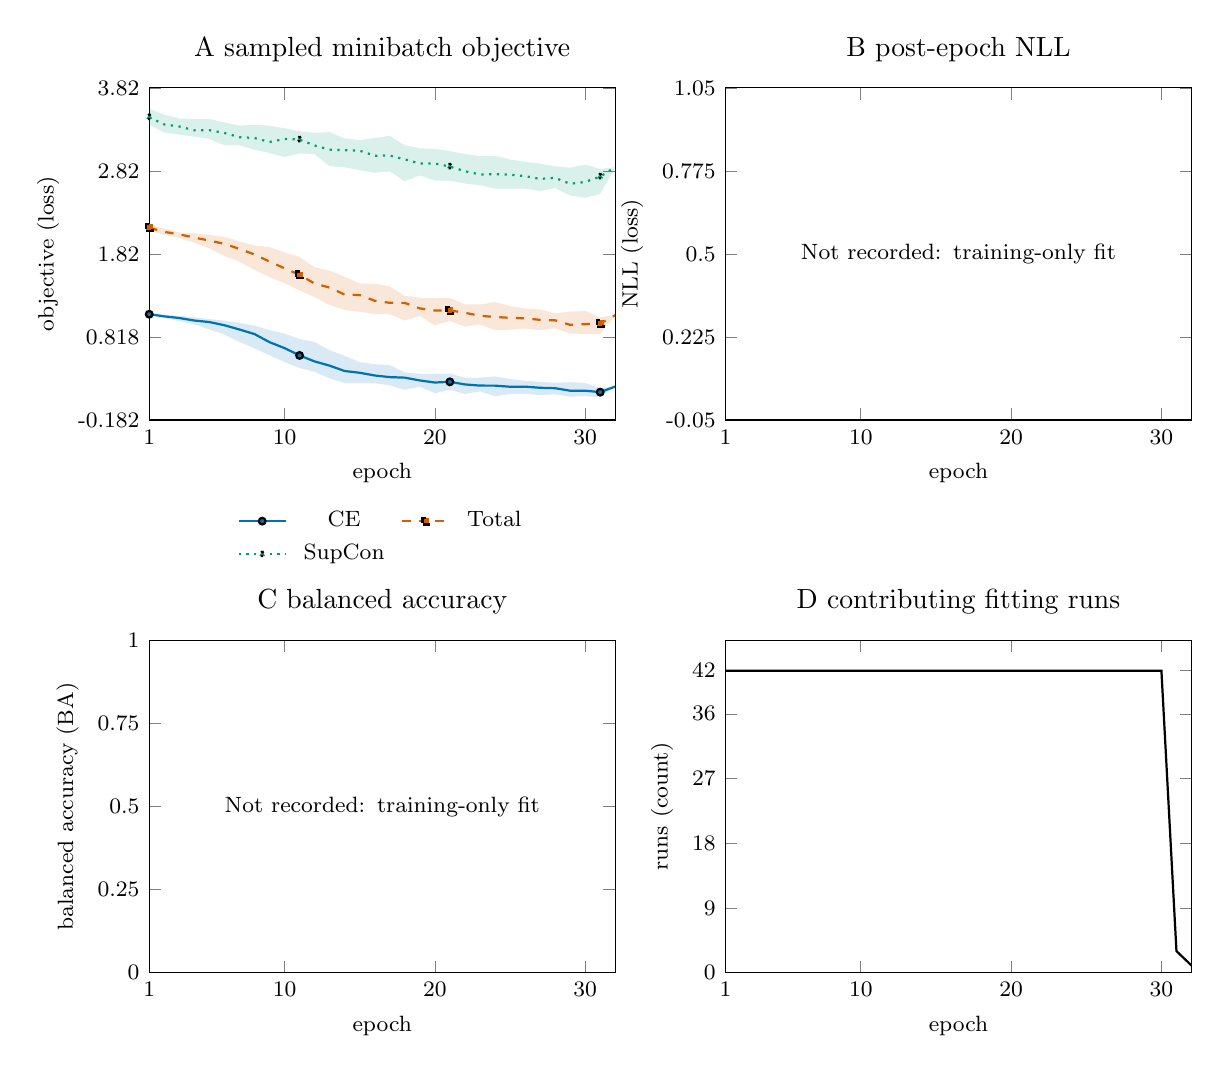
\begin{tikzpicture}
\begin{groupplot}[group style={group size=2 by 2, horizontal sep=14mm, vertical sep=28mm}]
\nextgroupplot[width=75mm, height=58mm, title={A sampled minibatch objective}, xlabel={epoch}, ylabel={objective (loss)}, xmin=1, xmax=32, xtick={1,10,20,30}, ymin=-0.18180758893489837, ymax=3.8179593676328656, ytick={-0.18180758893489837,0.81813415020704261,1.8180758893489835,2.8180176284909244,3.8179593676328656}, yticklabels={-0.182,0.818,1.82,2.82,3.82}, tick label style={font=\fontsize{8}{9}\selectfont, text=black}, label style={font=\fontsize{8}{9}\selectfont, text=black}, title style={font=\fontsize{10}{11}\selectfont, text=black}, legend style={at={(0.5,-0.24)},anchor=north,draw=none,fill=none,font=\fontsize{8}{9}\selectfont,row sep=1pt,column sep=4pt,legend columns=2}]
\addplot[fill=oi-blue,opacity=0.15,draw=none,forget plot] coordinates {(1,1.0821044832468032) (2,1.0475224494934081) (3,1.0103145152330399) (4,0.97122107297182081) (5,0.90728190094232564) (6,0.84839053601026537) (7,0.75786436498165133) (8,0.68035649806261067) (9,0.59790493696928027) (10,0.51599967926740642) (11,0.44461752399802207) (12,0.40026998370885847) (13,0.32001418024301531) (14,0.26125361248850826) (15,0.2596502173691988) (16,0.2610707849264145) (17,0.23654458913952112) (18,0.18252953793853521) (19,0.21871617585420608) (20,0.14050211478024721) (21,0.18185605704784394) (22,0.13227257058024408) (23,0.16333185862749816) (24,0.10508905686438084) (25,0.13052267339080573) (26,0.13287275210022925) (27,0.1188223073258996) (28,0.1271621908992529) (29,0.099835672974586495) (30,0.10648010559380054) (31,0.090723158419132227) (32,0.22198453918099403) (32,0.22198453918099403) (31,0.20254626125097275) (30,0.26410850808024405) (29,0.27358787953853603) (28,0.26772490218281747) (27,0.27808903418481351) (26,0.29000746384263038) (25,0.31252256333827971) (24,0.34352000690996642) (23,0.32748540937900544) (22,0.32652740254998208) (21,0.37871521338820457) (20,0.37545616403222082) (19,0.37525555565953256) (18,0.39213794767856597) (17,0.47918334156274794) (16,0.49101082980632782) (15,0.51486170366406436) (14,0.59153240621089931) (13,0.66013629883527758) (12,0.75849312841892236) (11,0.79426877498626713) (10,0.8590569943189621) (9,0.90203957408666613) (8,0.95385417342185974) (7,0.98910654783248897) (6,1.0142740309238434) (5,1.0339632660150528) (4,1.0557503432035447) (3,1.0708994299173356) (2,1.0849197238683701) (1,1.1008901178836823)};
\addplot[color=oi-blue, mark=*, mark options={draw=black}, mark repeat=10, mark size=1.2pt, solid, line width=0.8pt] coordinates {(1,1.0922608822584152) (2,1.0667595714330673) (3,1.0465438812971115) (4,1.0163880288600922) (5,0.99802248924970627) (6,0.95977098494768143) (7,0.90830361843109131) (8,0.85368799418210983) (9,0.75594452768564224) (10,0.6844925731420517) (11,0.59602762386202812) (12,0.52398151531815529) (13,0.47298890352249146) (14,0.40836869180202484) (15,0.38746391236782074) (16,0.3545396476984024) (17,0.33507217280566692) (18,0.32856497541069984) (19,0.29477528855204582) (20,0.26990877091884613) (21,0.27833282761275768) (22,0.2469785250723362) (23,0.2329765148460865) (24,0.23233664035797119) (25,0.21920977998524904) (26,0.22035037539899349) (27,0.20654475502669811) (28,0.20157510787248611) (29,0.17118309997022152) (30,0.17155456449836493) (31,0.15412699431180954) (32,0.22198453918099403)};
\addlegendentry{CE}
\addplot[fill=oi-vermillion,opacity=0.15,draw=none,forget plot] coordinates {(1,2.1007804036140443) (2,2.0476183831691741) (3,2.0110778689384459) (4,1.9538616508245468) (5,1.8845755070447923) (6,1.7926326632499694) (7,1.7259754806756973) (8,1.6251820474863052) (9,1.5424919039011002) (10,1.4657921701669694) (11,1.3798216700553894) (12,1.2969434827566146) (13,1.2031547635793687) (14,1.1411315947771072) (15,1.1226638615131379) (16,1.0941281631588935) (17,1.091882872581482) (18,1.0165139943361283) (19,1.0702349096536636) (20,0.95830181688070293) (21,1.0114162862300873) (22,0.94247450679540634) (23,0.96943874210119252) (24,0.90178308784961703) (25,0.90510814040899279) (26,0.92040305882692341) (27,0.90049557834863658) (28,0.92132136970758438) (29,0.86128093600273137) (30,0.85383271872997279) (31,0.85261441767215729) (32,1.0807514488697052) (32,1.0807514488697052) (31,1.0552047520875931) (30,1.1312447607517242) (29,1.1244691550731658) (28,1.1011458039283752) (27,1.1494506865739822) (26,1.1611124753952027) (25,1.1895402759313582) (24,1.2402078002691268) (23,1.2095775961875916) (22,1.211345911026001) (21,1.2878094524145127) (20,1.284194180369377) (19,1.2909829527139665) (18,1.3138874232769013) (17,1.4265881538391114) (16,1.4613379776477813) (15,1.4631697475910186) (14,1.5435772269964219) (13,1.6169749438762664) (12,1.6576358735561372) (11,1.7832793593406677) (10,1.835664415359497) (9,1.901737105846405) (8,1.9211225658655167) (7,1.9695270568132401) (6,2.0240940123796465) (5,2.0475419580936434) (4,2.0659880816936491) (3,2.0764451205730436) (2,2.1249922096729277) (1,2.1633811235427856)};
\addplot[color=oi-vermillion, mark=square*, mark options={draw=black}, mark repeat=10, mark size=1.2pt, dashed, line width=0.8pt] coordinates {(1,2.1342697739601135) (2,2.0841466784477234) (3,2.0540234446525574) (4,2.0156019777059555) (5,1.9790502488613129) (6,1.9401732832193375) (7,1.8786159008741379) (8,1.8124276697635651) (9,1.7266677469015121) (10,1.6450158655643463) (11,1.5664195865392685) (12,1.4615703672170639) (13,1.4130253344774246) (14,1.3289717584848404) (15,1.3232145607471466) (16,1.2542953640222549) (17,1.2298763692378998) (18,1.2285905778408051) (19,1.1625429391860962) (20,1.1366108953952789) (21,1.137813612818718) (22,1.1100480630993843) (23,1.0731875374913216) (24,1.0595883131027222) (25,1.0485308170318604) (26,1.0436111241579056) (27,1.0243852213025093) (28,1.0190059840679169) (29,0.96372795850038528) (30,0.97311180830001831) (31,0.97901220619678497) (32,1.0807514488697052)};
\addlegendentry{Total}
\addplot[fill=oi-green,opacity=0.15,draw=none,forget plot] coordinates {(1,3.3727055013179781) (2,3.2817234933376311) (3,3.2546032488346102) (4,3.2309207439422609) (5,3.2036925971508028) (6,3.1253446221351622) (7,3.1254507184028624) (8,3.0731010377407073) (9,3.0332139849662783) (10,2.9859151124954222) (11,3.0301500022411347) (12,3.0175917804241181) (13,2.8750337660312653) (14,2.8617318689823152) (15,2.8263857305049895) (16,2.7953497529029847) (17,2.8123373270034788) (18,2.6931995689868926) (19,2.7632934749126434) (20,2.7013709962368013) (21,2.6997336387634276) (22,2.6650998175144194) (23,2.6465808629989622) (24,2.6052958965301514) (25,2.6038189470767974) (26,2.6048546969890594) (27,2.5753740191459658) (28,2.6125689208507539) (29,2.5227195799350737) (30,2.4945000886917112) (31,2.5396374464035034) (32,2.8625562787055969) (32,2.8625562787055969) (31,2.8421948194503783) (30,2.8943771779537202) (29,2.8561208307743073) (28,2.8717364013195037) (27,2.9057462751865386) (26,2.9266682684421541) (25,2.955153149366379) (24,2.9984842538833618) (23,2.9968961775302887) (22,3.0226410031318665) (21,3.0564559638500213) (20,3.0827991724014283) (19,3.0900937438011167) (18,3.1277275323867797) (17,3.2400093078613281) (16,3.2148388743400571) (15,3.1892972826957702) (14,3.2101802825927734) (13,3.284480905532837) (12,3.2774898231029512) (11,3.2965364336967466) (10,3.3306995809078215) (9,3.3615106642246246) (8,3.3737818896770477) (7,3.3628927350044249) (6,3.4022281944751738) (5,3.4438073217868803) (4,3.4434297442436219) (3,3.4486998021602631) (2,3.4943737447261811) (1,3.5667062222957613)};
\addplot[color=oi-green, mark=triangle*, mark options={draw=black}, mark repeat=10, mark size=1.2pt, dotted, line width=0.8pt] coordinates {(1,3.4640264511108398) (2,3.3777123093605042) (3,3.3530651926994324) (4,3.3063473403453827) (5,3.3085135221481323) (6,3.2747490108013153) (7,3.2245135605335236) (8,3.2144042551517487) (9,3.1661855578422546) (10,3.2026870250701904) (11,3.1958138942718506) (12,3.1237576603889465) (13,3.0744990110397339) (14,3.0677819848060608) (15,3.0616979598999023) (16,3.0014258325099945) (17,3.0031096637248993) (18,2.957167774438858) (19,2.9067469835281372) (20,2.9068378508090973) (21,2.8706133663654327) (22,2.8148002624511719) (23,2.7751856446266174) (24,2.7785459756851196) (25,2.7719924449920654) (26,2.755278468132019) (27,2.7218440473079681) (28,2.7340544462203979) (29,2.6626682281494141) (30,2.6852649450302124) (31,2.7496172189712524) (32,2.8625562787055969)};
\addlegendentry{SupCon}
\nextgroupplot[width=75mm, height=58mm, title={B post-epoch NLL}, xlabel={epoch}, ylabel={NLL (loss)}, xmin=1, xmax=32, xtick={1,10,20,30}, ymin=-0.050000000000000003, ymax=1.05, ytick={-0.050000000000000003,0.22500000000000003,0.5,0.77500000000000002,1.05}, yticklabels={-0.05,0.225,0.5,0.775,1.05}, tick label style={font=\fontsize{8}{9}\selectfont, text=black}, label style={font=\fontsize{8}{9}\selectfont, text=black}, title style={font=\fontsize{10}{11}\selectfont, text=black}]
\node[align=center, text width=55mm, font=\fontsize{8}{9}\selectfont] at (axis cs:16.5,0.5) {Not recorded: training-only fit};
\nextgroupplot[width=75mm, height=58mm, title={C balanced accuracy}, xlabel={epoch}, ylabel={balanced accuracy (BA)}, xmin=1, xmax=32, xtick={1,10,20,30}, ymin=0, ymax=1, ytick={0,0.25,0.5,0.75,1}, yticklabels={0,0.25,0.5,0.75,1}, tick label style={font=\fontsize{8}{9}\selectfont, text=black}, label style={font=\fontsize{8}{9}\selectfont, text=black}, title style={font=\fontsize{10}{11}\selectfont, text=black}]
\node[align=center, text width=55mm, font=\fontsize{8}{9}\selectfont] at (axis cs:16.5,0.5) {Not recorded: training-only fit};
\nextgroupplot[width=75mm, height=58mm, title={D contributing fitting runs}, xlabel={epoch}, ylabel={runs (count)}, xmin=1, xmax=32, xtick={1,10,20,30}, ymin=0, ymax=46.200000000000003, ytick={0,9,18,27,36,42}, yticklabels={0,9,18,27,36,42}, tick label style={font=\fontsize{8}{9}\selectfont, text=black}, label style={font=\fontsize{8}{9}\selectfont, text=black}, title style={font=\fontsize{10}{11}\selectfont, text=black}]
\addplot[color=oi-black, solid, line width=0.8pt] coordinates {(1,42) (2,42) (3,42) (4,42) (5,42) (6,42) (7,42) (8,42) (9,42) (10,42) (11,42) (12,42) (13,42) (14,42) (15,42) (16,42) (17,42) (18,42) (19,42) (20,42) (21,42) (22,42) (23,42) (24,42) (25,42) (26,42) (27,42) (28,42) (29,42) (30,42) (31,3) (32,1)};
\end{groupplot}
\end{tikzpicture}
\par\vspace{6mm}
\begin{minipage}{175mm}
{\fontsize{8}{10}\selectfont RQ-S01 / Scope E: descriptive training diagnostics. 400-1800 cm-1 inputs: SG uses impulse replacement and Savitzky-Golay smoothing; arPLS uses impulse replacement and baseline correction; both finish with [0,1] min-max scaling. CE = chemical cross-entropy; SupCon = supervised contrastive; Paired = paired consistency; NLL = negative log-likelihood; BA = balanced accuracy. Authenticated complete monitor histories aggregated across unique fitting jobs into descriptive policy/recipe/stage curves. Curves summarize per-epoch minibatch-weighted training chemical cross-entropy and the composite total optimization objective; these sampled minibatch objectives differ from post-epoch evaluation negative log-likelihood. Auxiliary supcon/paired loss components are recipe-specific and are not directly comparable to the total objective across recipes. Validation metrics are recorded for source\_fit runs only and never substitute for a held-out test set; calibration\_model\_fit and final\_refit rows carry training-only diagnostics. Source\_fit optimization uses a 30-epoch minimum stopping threshold and a 200-epoch maximum; refit stages reuse the caller-selected duration. Curves are fitting-run-weighted descriptive summaries over correlated runs (seeds/splits). Lines show medians; 10th/90th percentiles describe variation among saved fitting runs, not confidence intervals. Only runs that reached each epoch contribute; early stopping changes the composition, and stopped runs are not carried forward. Fitting jobs are not independent chemical samples: the dataset has 598 spectra from 69 physical samples and 10 instruments. Coverage is limited to saved SG/arPLS monitor histories; historical MIN losses are not pooled or invented. A missing history is not a zero loss or proof of a failed model. These curves do not support hypothesis tests, superiority claims, model selection, or new uncertainty inference. P08 learned-method performance is reported elsewhere.}
\end{minipage}
\end{minipage}
\end{document}